% !TEX encoding = IsoLatin9

% !TEX encoding = IsoLatin9
\documentclass[aspectratio=54, 9pt]{beamer}
\usetheme[progressbar=frametitle]{metropolis}
\usepackage{graphicx}
\usepackage{xcolor}

% Define los colores del MIDE
\definecolor{rojito}{RGB}{178, 18, 18}    % Rojo UAEH
\definecolor{uaehred}{RGB}{49,163,84}    % Rojo UAEH
\definecolor{uaehgray}{RGB}{128, 128, 128} % Gris UAEH

% Aplica los colores al tema Metropolis
\setbeamercolor{alerted text}{fg=uaehred}
\setbeamercolor{frametitle}{bg=uaehred, fg=white}
\setbeamercolor{title separator}{fg=uaehred}
\setbeamercolor{progress bar}{fg=uaehred, bg=uaehgray}
\setbeamercolor{block title}{bg=uaehred, fg=white}
\setbeamercolor{block body}{bg=uaehgray!20, fg=black}
\setbeamercolor{background canvas}{bg=white}

\usepackage{calrsfs} % Paquete necesario para \mathcal


\usepackage{appendixnumberbeamer}
\usepackage{booktabs}
\usepackage[sfdefault]{FiraSans} %% option 'sfdefault' activates Fira Sans as the default text font
\usepackage[T1]{fontenc}
\renewcommand*\oldstylenums[1]{{\firaoldstyle #1}}
\newcommand\norm[1]{\left\lVert#1\right\rVert}           %% simbolo de la norma
\usepackage{mwe}     % For dummy images
\usepackage{lmodern} % To suppress some warnings
%-----------------------------------------------------------------
%-----------------------------------------------------------------
% Algunos paquetes.
\usepackage[spanish, mexico]{babel}
\usepackage[latin1]{inputenc}
\usepackage{amsthm}
\usepackage{enumerate}
\usepackage{amsmath}
\usepackage{hyperref}
\usepackage{subfig}                                            
\usepackage{tikz}
\usepackage{ragged2e}
\setbeamertemplate{bibliography item}[text] % a�adir referencias sin citarlas
\usepackage{appendixnumberbeamer}
\justifying
\setbeamercolor{math text}{fg=rojito}
\usepackage{pgf,tikz}
\usepackage{multirow}                      %%Para unir filas en tablas
\usetikzlibrary{arrows}
\newtheorem{defi}{Definici�n}
\newtheorem{teo}{Teorema}
\newtheorem{prop}{Proposici�n}
\RequirePackage{xcolor}
%\usecolortheme[RGB={99,99,99}]{structure} 
\definecolor{OwlRed}{RGB}{222,45,38}
\definecolor{OwlGreen}{RGB}{90, 168, 0}
\definecolor{OwlBlue}{RGB}{49,130,189}
\definecolor{OwlYellow}{RGB}{ 242, 147,  24}
\newcommand{\azul}[1]{\textcolor{OwlBlue}{#1}}
\newcommand{\amarillo}[1]{\textcolor{OwlYellow}{#1}}
\newcommand{\rojo}[1]{\textcolor{OwlRed}{#1}}
\newcommand{\verde}[1]{\textcolor{OwlGreen}{#1}}
\newcommand{\bs}[1]{\boldsymbol{#1}}

\usepackage{multicol}
\usepackage{multirow}
%\usepackage[table,xcdraw]{xcolor}


\usepackage{listings}
\definecolor{codegreen}{rgb}{0,0.6,0}
\definecolor{codegray}{rgb}{0.5,0.5,0.5}
\definecolor{codepurple}{rgb}{0.58,0,0.82}
\definecolor{backcolour}{rgb}{0.95,0.95,0.92}

\lstdefinestyle{mystyle}{
    backgroundcolor=\color{backcolour},   
    commentstyle=\color{codegreen},
    keywordstyle=\color{magenta},
    numberstyle=\tiny\color{codegray},
    stringstyle=\color{codepurple},
    basicstyle=\ttfamily\footnotesize,
    breakatwhitespace=false,         
    breaklines=true,                 
    captionpos=b,                    
    keepspaces=true,                 
    numbers=left,                    
    numbersep=5pt,                  
    showspaces=false,                
    showstringspaces=false,
    showtabs=false,                  
    tabsize=2
}

\lstset{style=mystyle}

% redefiniciones de comandos
% Definiciones de comandos personalizados
\newcommand{\be}{\begin{equation*}}
\newcommand{\ee}{\end{equation*}}

\newcommand{\bi}{\begin{itemize}}
\newcommand{\ei}{\end{itemize}}


%-----------------------------------------------------------------
%-----------------------------------------------------------------
\begin{document}

\title[Tema]{Raz�n de cambio}
\subtitle{Preliminares}
\author{Dr. Bartolo de Jes�s Villar-Hern�ndez} 
\date{\today} 
\institute{``Far better an approximate answer to the right question, which is 
often vague, than the exact answer to the wrong question, which can
always be made precise''  (John Tukey, Ann. Math. Stat. [33] 1962)}
\titlegraphic{\hfill
\includegraphics[height=3.0cm]{logo/mide.png}}

%-----------------------------------------------------------------
%-----------------------------------------------------------------
\begin{frame}[plain]
  \titlepage
\end{frame}


%-----------------------------------------------------------------
%-----------------------------------------------------------------
%\begin{frame}{Contenido}
%\transwipe
%\tableofcontents
%\end{frame}

%-----------------------------------------------------------------
%-----------------------------------------------------------------

%-------
\begin{frame}{Introducci�n}

La concentraci�n promedio anual de $CO_2$ atmosf�rico en Mauna Loa\footnote{\url{https://es.wikipedia.org/wiki/Mauna_Loa}}, en partes por mill�n (ppm), $t$ a�os despu�s de 1950, est� dada por la siguiente funci�n:

\be
\text{CO}_{2(t)} = 0.0134594696825t^2 + 0.520632601929t + 310.423363171
\ee

Para comprender c�mo han cambiado y est�n cambiando los niveles de CO\(_2\), planteamos dos preguntas. 

\bi
\item �qu� tan r�pido estaba aumentando el CO\(_2\) desde 1950 hasta 2017
\item �qu� tan r�pido est�n aumentando los niveles de CO\(_2\) en 2017?
\ei

\end{frame}

%-------
\begin{frame}{Intro...}

\centering 
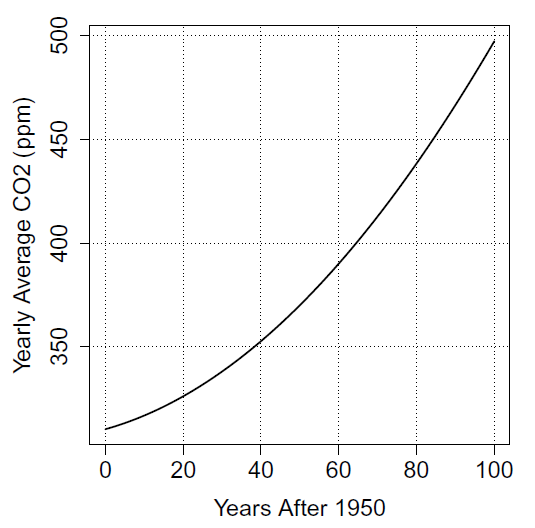
\includegraphics[width=0.75\textwidth]{./img/Fig1.PNG}

\end{frame}

%--------
\begin{frame}{Introducci�n}

Antes de contestar las interrogantes, vamos a plantear algunas definiciones.

\begin{block}{Pendiente de una l�nea secante}
La pendiente de una l�nea secante desde $(a, f(a))$ hasta $(b, f(b))$ es

\be
\frac{f(b)-f(a)}{b-a}
\ee

Tambi�n es la raz�n de cambio promedio de una funci�n desde $x=a$ hasta $x=b$.
\end{block}
\end{frame}

%-------
\begin{frame}{Ejemplo}

\textbf{\rojo{Ejercicio}}

Suponga que $R(x) = 100x - 4x^2$ es el ingreso en d�lares por la venta de $x$ widgets. Calcule e interprete la pendiente de la recta secante desde $x = 5$ hasta $x = 10$.

En promedio, los ingresos aumentaron 40 d�lares por widget cuando el n�mero de widgets vendidos aument� de 5 a 10 widgets.

\pause

\textbf{\azul{Soluci�n}}

$R(10) = 100(10) - 4(10^2) = \$ 600$

$R(5) = 100(5) - 4(5^2) = \$ 400$


Sustituyendo

$$
\frac{\$ 600 - \$ 400}{10 \text{widgets} - 5 \text{widgets}} = 40 \text{d�lares/widgets}
$$

\end{frame}





%-------
\begin{frame}[fragile]{En R}

\begin{verbatim}
\end{verbatim}
  > CO2<-function(t){0.0134594696825104*t?2+
        0.520632601928747*t+310.423363171355}
        > a<-0
        > b<-67
        > (CO2(b)-CO2(a))/(b-a)
\end{frame}


%-------
%\begin{frame}{}
%\end{frame}


%-------
%\begin{frame}{}
%\end{frame}


%-------
%\begin{frame}{}
%\end{frame}

%-------
%\begin{frame}{}
%\end{frame}


%-------
%\begin{frame}{}
%\end{frame}



%-------
%\begin{frame}{}
%\end{frame}


%-------
%\begin{frame}{}
%\end{frame}

%-------
%\begin{frame}{}
%\end{frame}


%-----------------------------------------------------------------
%-----------------------------------------------------------------


%-----------------------------------------------------------------
%-----------------------------------------------------------------

%-----------------------------------------------------------------
%-----------------------------------------------------------------
%{\setbeamercolor{palette primary}{fg=white, bg=black}
%\begin{frame}[standout]
%  ?Preguntas?
%\end{frame}
%}

%-----------------------------------------------------------------
%-----------------------------------------------------------------
%\begin{frame}[standout]
%  ?Gracias!
%\end{frame}
%-----------------------------------------------------------------
\end{document}
%-----------------------------------------------------------------
%-----------------------------------------------------------------